\documentclass[11pt,a4paper]{article}
\usepackage[T1]{fontenc}
\usepackage{lmodern}
\usepackage[a4paper,margin=1in]{geometry}
\usepackage{amsmath,amssymb,amsthm}
\usepackage{booktabs}
\usepackage{tikz}
\usepackage[hidelinks,pdftitle={A counterexample to Conjecture 399b of Written on the Wall II},pdfauthor={Jiri Chmel}]{hyperref}
\usepackage{xurl}

\newtheorem{theorem}{Theorem}
\newtheorem{lemma}[theorem]{Lemma}
\newtheorem{conjecture}{Conjecture}
\renewcommand{\theconjecture}{399b}
\theoremstyle{definition}
\newtheorem{definition}[theorem]{Definition}
\theoremstyle{remark}
\newtheorem{remark}[theorem]{Remark}

\newcommand{\Gc}{\overline{G}}
\newcommand{\WP}{\operatorname{WP}}
\newcommand{\flr}[1]{\lfloor #1\rfloor}

\title{A counterexample to Conjecture 399b of Written on the Wall II}
\author{Ji\v{r}\'{\i} Chmel}
\date{22 November 2026\\[1ex]
\small Preprint, version 1. It has not yet been fully reviewed by the author;\\
a version reviewed by the author will follow.}

\begin{document}
\maketitle

\begin{abstract}
Conjecture 399b of Written on the Wall II, a list of conjectures made by the program Graffiti.pc,
states that every connected graph $G$ on $n>2$ vertices satisfies
$\gamma_2(G)\le\WP(\Gc)+\flr{3/\alpha(G[A_3])}$. Here $\gamma_2$ is the 2-domination number,
$\WP(\Gc)$ is the Welsh--Powell invariant of the complement, and $A_3$ is the set of vertices of
degree at least three. DeLaVi\~na and Pepper proved $\gamma_2(G)\le\WP(\Gc)+1$, which settles
every graph with $1\le\alpha(G[A_3])\le 3$. We show that the conjecture is false in the remaining
case. For every $q\ge 3$ we give a connected graph $F_q$ on $q+9$ vertices with
$\gamma_2(F_q)=7$, $\WP(\overline{F_q})=6$ and $\alpha(F_q[A_3])=4$. The proof is elementary, and
it has also been checked in the Lean proof assistant. The smallest member of the family has 12
vertices, and exhaustive computer searches show that, with the catalogue's reading of the
Welsh--Powell invariant, no counterexample has 11 or fewer.
\end{abstract}

\section{Introduction}

Written on the Wall II~\cite{wowii} is E.~DeLaVi\~na's list of conjectures made by her program
Graffiti.pc~\cite{gpc}. Early in a run of January 2010 the program conjectured
$\gamma_2(G)\le\WP(\Gc)+1$, and later in the run it added entries 399a and 399b, which try to say
when the $+1$ can be dropped; entry 399c, also of January 2010, is a third bound of the same kind.
The definitions are recalled in Section~\ref{sec:defs}.

\begin{conjecture}[\cite{wowii}]
If $G$ is a connected graph on $n>2$ vertices, then
\[
\gamma_2(G)\le\WP(\Gc)+\flr{3/\alpha(G[A_3])},
\]
where $A_3$ is the set of vertices of degree at least three.
\end{conjecture}

In 2012 DeLaVi\~na and Pepper~\cite{dp12} proved $\alpha_k(G)\le\WP(\Gc)+k-1$ for every graph and
every $k\ge 1$ (their Theorem~2.1), where $\alpha_k$ is the $k$-independence number. With
Favaron's inequality $\gamma_k\le\alpha_k$~\cite{favaron} this gives
$\gamma_2(G)\le\alpha_2(G)\le\WP(\Gc)+1$ (their Corollary~2.2), which settles the conjecture made
early in the run, Conjecture~4 of~\cite{dlpw}. Since $\flr{3/a}\ge 1$ for
$a=1,2,3$, Conjecture~399b follows whenever $1\le\alpha(G[A_3])\le 3$. As the catalogue's note of
May 2012 says, it remains to show $\gamma_2(G)\le\WP(\Gc)$ for connected graphs with
$\alpha(G[A_3])\ge 4$. (For graphs of maximum degree at most two, $A_3$ is empty and the right side
is undefined; such graphs play no role here.) In the latest states of the catalogue that we could
see, an Internet Archive capture of 26 July 2026 and a copy of its rows that AI Village committed on
1 September 2026~\cite{aiv}, the entry is marked open; see the section on sources and status at the
end.

We show that this remaining case fails.

\begin{theorem}\label{thm:main}
For every integer $q\ge 3$ the graph $F_q$ of Definition~\ref{def:F} is connected, has $q+9$
vertices, and satisfies
\[
\gamma_2(F_q)=7,\qquad \WP(\overline{F_q})=6,\qquad \alpha(F_q[A_3])=4 .
\]
Hence $\gamma_2(F_q)=7>6=\WP(\overline{F_q})+\flr{3/\alpha(F_q[A_3])}$, and Conjecture~399b is
false.
\end{theorem}

Since $\gamma_2\le\WP(\Gc)+1$ always holds, every counterexample violates the bound by exactly
one, has $\alpha(G[A_3])\ge 4$, and has $\gamma_2(G)=\alpha_2(G)=\WP(\Gc)+1$. The graphs $F_q$ are
of this kind (Remark~\ref{rem:tight}).

\emph{Earlier work.} Neither~\cite{dlpw} nor~\cite{dp12} mentions entry 399b; its reduction to the
case $\alpha(G[A_3])\ge 4$ is the catalogue's note. We know of two computational studies of the
entry. In 2026 agents of the AI Village project scanned the open entries of the
catalogue~\cite{aiv}. For 399b they found the bound attained but never violated on connected graphs
with at most nine vertices, and they reported that hill-climbing at order~12 found graphs with
$\gamma_2=\WP(\Gc)+1$ and $\alpha(G[A_3])=2$, but none with larger $\alpha(G[A_3])$. Their counts
of graphs with $\gamma_2=\WP(\Gc)+1$ agree with ours, but they also reported that no such graph on
at most nine vertices has $\alpha(G[A_3])\ge 3$. That is not correct: the graph obtained from
$K_{3,3}$, with parts $\{u_1,u_2,u_3\}$ and $\{v_1,v_2,v_3\}$, by adding the edge $u_2u_3$ and a
pendant vertex at each of $v_2$ and $v_3$ has eight vertices, $\gamma_2=5=\WP(\Gc)+1$ and
$\alpha(G[A_3])=3$.\footnote{Call the pendant vertices $p$ (at $v_2$) and $r$ (at $v_3$). The
degrees are $1,1,3,3,4,4,4,4$, so $\WP(\Gc)=4$, and $\alpha(G[A_3])=3$, because an independent set
of $K_{3,3}$ lies in one part and $u_2u_3$ is an edge. The set $\{p,r,v_1,v_2,v_3\}$ is
2-dominating. Let $D$ be 2-dominating, so that $p,r\in D$, and suppose that $D'=D\setminus\{p,r\}$
has at most two vertices. If $v_1\notin D$, then $D'$ consists of two of $u_1,u_2,u_3$, and the
third has at most one neighbour in $D$. So $v_1\in D$. If $u_1\in D$, then $D'=\{u_1,v_1\}$ and
$u_2$ has only $v_1$ in $D$. Otherwise $u_1$ needs $v_2$ or $v_3$ in $D$, say $v_2$ (exchanging
$v_2$ with $v_3$ and $p$ with $r$ is an automorphism); then $D'=\{v_1,v_2\}$ and $v_3$ has only $r$
in $D$. Hence $\gamma_2=5$.} The repository
c5-k4~\cite{c5k4} lists 399b as open and records it as holding on fifty strongly regular and
related graphs, with the Welsh--Powell invariant computed from the degrees of the complement (the
other reading of Section~\ref{sec:defs}). The sibling entries 399a and 399c were refuted by AI
Village in August 2026, 399a with graphs as small as $K_3$ and $P_4$~\cite{aiv}. We found no other
work on 399b. The end of the paper lists the sources we consulted.

\subsection{Use of generative AI}\label{sec:ai}

The counterexample was found, and this paper was written, by Claude Opus~5.5, a generative AI
system made by Anthropic, on 21 and 22 November 2026, in sessions directed by the author. Claude
was used through Claude Code, Anthropic's agentic coding tool. The author asked for work on open
conjectures of Graffiti.pc, set the working rules, and decided which lines of work to pursue and
which results to write up. Claude agents scanned the open entries of the catalogue and singled out
entry 399b. Claude searched for counterexamples, found the family $F_q$ and the proof of
Theorem~\ref{thm:main}, wrote the programs and the formal proof described in
Section~\ref{sec:verify}, and drafted the text. The graph generator of one of those programs comes
from a library that Claude Fable~5.2, another Anthropic model, wrote in this project on
19 November 2026. Further Claude instances, writing programs of their
own, refereed the proof by hand, recomputed the invariants, repeated the searches, audited the
formal proof and checked the status of the conjecture in primary sources. None of this is external peer review. The Lean kernel's check of the formal proof does not depend
on any AI system; that the formal statement expresses Conjecture~399b was checked as described in
Section~\ref{sec:verify}. Claude is not an author. The author takes full responsibility for the
content of this paper. This first version is a preprint, posted on 22 November 2026 before the
author's own full review; a version reviewed by the author will replace it.

\section{Definitions and the reading of the statement}\label{sec:defs}

Graphs are finite and simple. For a graph $G=(V,E)$ with $n=|V|$ vertices, $N(v)$ is the
neighbourhood of a vertex $v$ and $d(v)=|N(v)|$ its degree. For $S\subseteq V$, $G[S]$ is the
induced subgraph, and $\alpha(H)$ is the independence number of a graph~$H$. The definitions below
are those of the catalogue's definitions file~\cite{wowii} (its definitions 90 and 113) and of
DeLaVi\~na and Pepper~\cite{dp12}.

\emph{2-domination}~\cite{fj,dlpw}. A set $D\subseteq V$ is \emph{2-dominating} if every vertex
outside $D$ has at least two neighbours in $D$. The \emph{2-domination number} $\gamma_2(G)$ is the
least size of a 2-dominating set. A vertex of degree one belongs to every 2-dominating set.

\emph{2-independence}~\cite{dp12}. The \emph{2-independence number} $\alpha_2(G)$ is the largest
size of a set $S$ such that $G[S]$ has maximum degree at most one. (DeLaVi\~na and Pepper write
$\beta_k$ for the $k$-independence number $\alpha_k$.)

\emph{The Welsh--Powell invariant of the complement.} Let $d_1\le d_2\le\dots\le d_n$ be the
degrees of~$G$ in nondecreasing order. Then
\[
\WP(\Gc)=\max\{\,k : k+d_k\le n\,\}.
\]
The maximum exists because $1+d_1\le n$. This is the catalogue's definition~113 and the
definition in Section~2 of~\cite{dp12}. The name comes from the Welsh--Powell bound
$\chi(H)\le\max_i\min\{i,\,\delta_i+1\}$, where $\delta_1\ge\delta_2\ge\dots$ are the degrees of
$H$ in nonincreasing order~\cite{wp}. For $H=\Gc$ we have $\delta_i=n-1-d_i$, and
$\max_i\min\{i,n-d_i\}=\WP(\Gc)$. To see this, let $k^*$ be the largest $k$ with $k+d_k\le n$.
For $i\le k^*$, $\min\{i,n-d_i\}=i\le k^*$, with equality at $i=k^*$. For $i>k^*$,
$n-d_i<i$, so $\min\{i,n-d_i\}=n-d_i\le n-d_{k^*+1}<k^*+1$.

\emph{Another reading.} Definition~113 does not say whose degree sequence is meant, and one could
apply the formula $\max\{k:k+d_k\le n\}$ to the degrees of $\Gc$ instead of those of $G$. That is
not the intended reading: DeLaVi\~na and Pepper~\cite{dp12} use the degrees of $G$, and their
Theorem~2.1 would fail under the other reading, since the star $K_{1,4}$ would get the value~2
while $\alpha_2(K_{1,4})=4>2+1$. AI Village made the same observation, using~\cite{dp12} and the
catalogue's proved entries 436a and 436b~\cite{aiv}. Under that reading 399b fails already for the star $K_{1,6}$ on seven
vertices: there $\gamma_2=6$, the degrees $0,5,5,5,5,5,5$ of the complement give the value~2, and
$\flr{3/\alpha(G[A_3])}=3$. No connected graph on six or fewer vertices fails under it
(Section~\ref{sec:verify}).
Remark~\ref{rem:reading} records what happens to $F_q$ under it.

\section{The counterexamples}\label{sec:proof}

\begin{definition}\label{def:F}
Let $q\ge 3$. The graph $F_q$ has the $q+9$ vertices
\[
x_1,x_2,x_3,\quad \ell_1,\ell_2,\ell_3,\quad k_1,\dots,k_q,\quad w,\quad y_1,y_2,
\]
and the following edges: $x_i\ell_i$ for $i=1,2,3$; all edges $k_ik_j$, so $K=\{k_1,\dots,k_q\}$
is a clique; all edges $x_ik_j$; all edges $wk_j$; and all edges $y_tx_i$ ($t=1,2$). We write
$X=\{x_1,x_2,x_3\}$ and $Y=\{y_1,y_2\}$. There are no other edges; in particular $X$ and $Y$ are
independent sets and $w$ has no neighbour outside~$K$.
\end{definition}

\begin{figure}[ht]
\centering
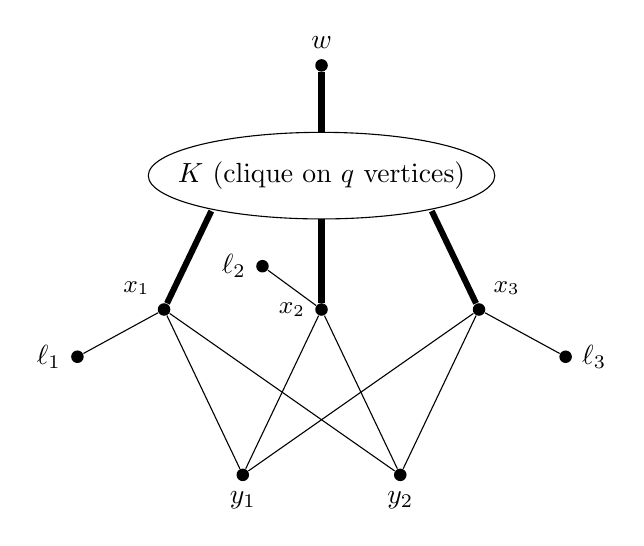
\begin{tikzpicture}[v/.style={circle,fill,inner sep=1.6pt},
                    lab/.style={font=\small}]
  \draw (0,2.3) ellipse (2.2 and 0.55);
  \node at (0,2.3) {$K$ (clique on $q$ vertices)};
  \node[v,label={above:$w$}] (w) at (0,3.7) {};
  \node[v,label={[lab]above left:$x_1$}] (x1) at (-2,0.6) {};
  \node[v,label={[lab]left:$x_2$}] (x2) at (0,0.6) {};
  \node[v,label={[lab]above right:$x_3$}] (x3) at (2,0.6) {};
  \node[v,label={left:$\ell_1$}] (l1) at (-3.1,0) {};
  \node[v,label={left:$\ell_2$}] (l2) at (-0.75,1.15) {};
  \node[v,label={right:$\ell_3$}] (l3) at (3.1,0) {};
  \node[v,label={below:$y_1$}] (y1) at (-1,-1.5) {};
  \node[v,label={below:$y_2$}] (y2) at (1,-1.5) {};
  \draw[line width=2.2pt] (w) -- (0,2.85);
  \draw[line width=2.2pt] (x1) -- (-1.4,1.85);
  \draw[line width=2.2pt] (x2) -- (0,1.75);
  \draw[line width=2.2pt] (x3) -- (1.4,1.85);
  \draw (x1) -- (l1) (x2) -- (l2) (x3) -- (l3);
  \foreach \y in {y1,y2} { \foreach \x in {x1,x2,x3} { \draw (\y) -- (\x); } }
\end{tikzpicture}
\caption{The graph $F_q$. A thick line means that the vertex is adjacent to every vertex of the
clique~$K$.}
\label{fig:F}
\end{figure}

The graph $F_q$ is connected: every vertex is adjacent to $K$ or to $X$, and $X$ is joined
to~$K$. Its degrees are
\[
d(\ell_i)=1,\quad d(y_t)=3,\quad d(w)=q,\quad d(x_i)=1+q+2=q+3,\quad d(k_j)=(q-1)+3+1=q+3 .
\]

\begin{lemma}\label{lem:wp}
$\WP(\overline{F_q})=6$.
\end{lemma}

\begin{proof}
Here $n=q+9$. Since $q\ge 3$, the degrees in nondecreasing order are $1,1,1,3,3,q$, followed by
$q+3$ entries equal to $q+3$. For $k=6$ we have $k+d_k=6+q\le n$. For every $k\ge 7$ we have
$d_k=q+3$ and $k+d_k\ge q+10>n$.
\end{proof}

\begin{lemma}\label{lem:alpha}
$A_3=X\cup K\cup\{w\}\cup Y$ and $\alpha(F_q[A_3])=4$.
\end{lemma}

\begin{proof}
The vertices of degree at least three are all vertices except the leaves $\ell_i$; note
$d(w)=q\ge 3$. The set $X\cup\{w\}$ is independent, so $\alpha(F_q[A_3])\ge 4$. Let $I\subseteq A_3$
be independent. If $I$ contains a vertex $k_j$ of $K$, then $I\subseteq\{k_j\}\cup Y$, because $k_j$
is adjacent to every other vertex of $X\cup K\cup\{w\}$; so $|I|\le 3$. Otherwise
$I\subseteq X\cup\{w\}\cup Y$. Every vertex of $X$ is adjacent to every vertex of $Y$, so $I$ misses
$X$ or misses $Y$, and $|I|\le\max\{|X\cup\{w\}|,|Y\cup\{w\}|\}=4$.
\end{proof}

\begin{lemma}\label{lem:gamma}
$\gamma_2(F_q)=7$.
\end{lemma}

\begin{proof}
\emph{Upper bound.} Let $D_0=\{\ell_1,\ell_2,\ell_3,x_1,x_2,x_3,w\}$. Each $y_t$ has its three
neighbours $x_1,x_2,x_3$ in $D_0$. Each $k_j$ has the four neighbours $x_1,x_2,x_3,w$ in $D_0$. So
$D_0$ is 2-dominating, and $\gamma_2(F_q)\le 7$.

\emph{Lower bound.} Let $D$ be a 2-dominating set. The leaves have degree one, so
$\ell_1,\ell_2,\ell_3\in D$. Write $a=|D\cap X|$, $b=|D\cap K|$, $e=|D\cap\{w\}|$ and $f=|D\cap Y|$.
It suffices to show $a+b+e+f\ge 4$. We use four observations.
\begin{enumerate}
\item[(i)] If $w\notin D$, then $w$ has two neighbours in $D$, all of them in $K$, so $b\ge 2$.
Hence $e=1$ or $b\ge 2$; in particular $b+e\ge 1$.
\item[(ii)] If some $y_t$ is not in $D$, then $y_t$ has two neighbours in $D$, all of them in $X$, so
$a\ge 2$.
Hence $a\le 1$ implies $f=2$.
\item[(iii)] If some $x_i\notin D$, then $x_i$ needs a neighbour in $D$ besides $\ell_i$, and its
other neighbours lie in $K\cup Y$. Hence $a\le 2$ implies $b+f\ge 1$.
\item[(iv)] If $a=0$ and $b=0$, then any vertex $k_j$ lies outside $D$ and its only possible
neighbour in $D$ is $w$, which is too few. Hence $a=0$ implies $b\ge 1$.
\end{enumerate}
Now distinguish the value of~$a$.
\begin{itemize}
\item $a=3$: by (i), $b+e\ge 1$, so $a+b+e+f\ge 4$.
\item $a=2$: if $b\ge 2$ we are done. Otherwise $e=1$ by (i), and $b+f\ge 1$ by (iii), so
$a+b+e+f\ge 2+1+1=4$.
\item $a=1$: $f=2$ by (ii) and $b+e\ge 1$ by (i), so $a+b+e+f\ge 1+1+2=4$.
\item $a=0$: $f=2$ by (ii). If $e=0$ then $b\ge 2$ by (i); if $e=1$ then $b\ge 1$ by (iv). In both
cases $b+e\ge 2$, and $a+b+e+f\ge 4$.
\end{itemize}
So $|D|=3+a+b+e+f\ge 7$.
\end{proof}

\begin{proof}[Proof of Theorem~\ref{thm:main}]
Connectivity and the order were noted after Definition~\ref{def:F}. By
Lemmas~\ref{lem:wp},~\ref{lem:alpha} and~\ref{lem:gamma},
$\WP(\overline{F_q})+\flr{3/\alpha(F_q[A_3])}=6+\flr{3/4}=6<7=\gamma_2(F_q)$.
\end{proof}

\begin{remark}\label{rem:tight}
By~\cite{dp12,favaron}, $7=\gamma_2(F_q)\le\alpha_2(F_q)\le\WP(\overline{F_q})+1=7$, so
$\alpha_2(F_q)=7$ as well; for instance $\{\ell_1,\ell_2,\ell_3,x_1,x_2,x_3,w\}$ induces three
disjoint edges and an isolated vertex. The graphs $F_q$ therefore attain the bound of DeLaVi\~na and
Pepper, and they show that no correction term that vanishes when $\alpha(G[A_3])\ge 4$ can replace
the $+1$.
\end{remark}

\begin{remark}\label{rem:why}
The construction separates the two sides of the inequality. The invariant $\WP(\overline{F_q})$
is pinned at~6 by the six vertices of small degree (three leaves, $y_1$, $y_2$ and $w$), whatever
the size of the clique. The leaves force themselves into every 2-dominating set, and the vertices
$w$, $y_1$, $y_2$, $x_1$, $x_2$, $x_3$ and the clique together force four more. Finally $X\cup\{w\}$ is an independent
set of four vertices of degree at least three, which makes the correction term vanish.
\end{remark}

\begin{remark}\label{rem:reading}
Under the other reading of Section~\ref{sec:defs}, with the degrees of $\Gc$, the invariant of
$\overline{F_q}$ becomes $q+3$. So $F_3$ is a counterexample under both readings, while $F_q$ with
$q\ge 4$ is a counterexample only under the catalogue's reading.

Two other variants of the definitions do not rescue the conjecture. A note on entry 391, added
to the catalogue after the capture of 26 July 2026 and recorded in the later copy of its
rows~\cite{aiv}, reports a counterexample sent on 24 July 2026. Entry 391 defines $A_3$ in the same
words as 399b, and in the note the catalogue's author suspects that $A_3$ should have been the set
of vertices of degree at most three. In $F_q$ these vertices are the
leaves, $y_1$, $y_2$, and also $w$ when $q=3$; they form an independent set of at least five
vertices, so the correction term is $0$ and the bound is still $6<7$. If ``adjacent to 2 vertices''
in definition~90 is read as ``adjacent to exactly two'', then the only such set in $F_q$ is the
whole vertex set, and the inequality fails by more. Indeed, let $D$ be such a set; the leaves lie
in $D$. If some $y_t$ were outside $D$, exactly two vertices of $X$ would lie in $D$, say not $x_1$.
A vertex $k_j$ outside $D$ would then already have two neighbours in $X\cap D$, so $D$ would contain
no vertex of $K$ and $w$ would have no neighbour in $D$; hence $K\subseteq D$, and then $x_1$ has
$\ell_1$ and the $q\ge 3$ vertices of $K$ in $D$, too many. So $Y\subseteq D$. Then each $x_i$ has
the three neighbours $\ell_i,y_1,y_2$ in $D$, so $X\subseteq D$; each $k_j$ has three neighbours in
$X$, so $K\subseteq D$; and $w$ has $q\ge 3$ neighbours in $D$, so $w\in D$.
\end{remark}

\begin{remark}\label{rem:order}
With the catalogue's reading of WP, the computer searches of Section~\ref{sec:verify} find no
connected graph on at most 11 vertices that violates Conjecture~399b, so $F_3$, with 12 vertices
and 24 edges, is a counterexample of minimum order. (Under the other reading $K_{1,6}$ already
fails; see Section~\ref{sec:defs}.) In graph6 format $F_3$ is
\begin{center}
\texttt{KCOfFFb?\textasciitilde?[?}
\end{center}
Deleting any single vertex or edge of $F_3$ gives a graph that is disconnected or satisfies the
conjecture with the catalogue's reading of WP; under the other reading, 21 of the 30 connected
ones violate it, for example $F_3-k_1$. Nor is $F_3$ the only counterexample on 12 vertices. Take
the complete graph on $u,v,c_1,\dots,c_6$ and delete the edge $uv$; add vertices $s_1,s_2,s_3$ with
$N(s_1)=\{u,v,c_5\}$, $N(s_2)=\{v,c_3,c_4\}$ and $N(s_3)=\{u,c_1,c_2\}$, and a leaf $\lambda$ at
$c_6$. This graph has 12 vertices and 37 edges, and its degrees are $1,3,3,3$ and eight times~$8$,
so $\WP(\Gc)=4$. An independent set contains at most two of $u,v,c_1,\dots,c_6$, and two only if
they are $u$ and $v$, which together see $s_1,s_2,s_3$; so $\alpha(G[A_3])=4$, attained by
$\{s_1,s_2,s_3,c_6\}$. The set $\{\lambda,s_1,s_2,s_3,c_6\}$ is 2-dominating. Conversely, let $D$ be
2-dominating with $|D|\le 4$, so that $\lambda\in D$, and let $t$ be the number of $s_i$ in $D$. If
$t=0$, the $s_i$ need six incidences with $D\setminus\{\lambda\}$, but its at most three vertices
give at most five, since only $u$ and $v$ lie in two of the sets $N(s_i)$. If $t=1$, the other two
$s_i$ need two common neighbours in $D$, but two of the sets $N(s_i)$ share at most one vertex. If
$t=2$, the third $s_i$ has at most one neighbour in $D$; if $t=3$, $c_6$ has only $\lambda$ in $D$.
Hence $\gamma_2=5>\WP(\Gc)+\flr{3/4}$.
\end{remark}

\section{Computational checks}\label{sec:verify}

The proof above is complete without computation. The following checks were made as well; the
programs and their output are in the supplement.
\begin{itemize}
\item \emph{The family.} For $q=3,\dots,10$, two programs that share no code computed
$\gamma_2$, $\alpha_2$, $\WP(\Gc)$ and $\alpha(G[A_3])$ of $F_q$, with identical results:
$7,7,6,4$ in every case. A third program, \texttt{verify\_399b.py} (Python standard library
only, brute force from the definitions), repeats the computation, checks that the two formulas for
$\WP(\Gc)$ in Section~\ref{sec:defs} agree, computes the other reading of
Remark~\ref{rem:reading}, and confirms that the graph6 string above encodes a graph isomorphic
to~$F_3$.
\item \emph{Small orders.} Two programs that share no code enumerated all connected graphs on $4$
to $10$ vertices (11,716,571 graphs on 10 vertices) and evaluated the conjecture on each; their
statistics agree in every field they share. A third, independently written program agrees. No graph
violates Conjecture~399b with the catalogue's reading. The numbers of graphs with
$\alpha(G[A_3])\ge 4$, the only ones for which the conjecture is not already a theorem, are 4, 286,
31,965 and 4,229,763 for $n=7,8,9,10$; a graph with $\alpha(G[A_3])\ge 4$ has four independent
vertices of degree at least three, hence at least seven vertices.
\item \emph{Eleven vertices.} With the catalogue's reading, no connected graph on 11 vertices
violates the conjecture. Let $v$ be a vertex of a graph $G$ on $n\ge 2$ vertices and $H=G-v$.
First, $\gamma_2(G)\le\gamma_2(H)+1$, since a 2-dominating set of $H$ together with $v$
2-dominates $G$. Second, $\WP(\overline{H})\le\WP(\Gc)\le\WP(\overline{H})+1$. Indeed $\WP(\Gc)$ is
the largest $k$ such that at least $k$ vertices of $G$ have degree at most $n-k$, and
$d_G(u)-1\le d_H(u)\le d_G(u)$ for $u\ne v$. If $k$ vertices of $H$ have degree at most
$(n-1)-k$ in $H$, they have degree at most $n-k$ in $G$; and if $k$ vertices of $G$ have degree at
most $n-k$, at least $k-1$ of them lie in $H$ and have degree at most $(n-1)-(k-1)$ there. Every
connected graph has a vertex that is not a cut vertex, for example a leaf of a spanning tree. So
every connected graph $G$ on 11 vertices with $\gamma_2(G)\ge\WP(\Gc)+1$, in particular every
counterexample, arises from a connected graph $H$ on 10 vertices with
$\gamma_2(H)\ge\gamma_2(G)-1\ge\WP(\Gc)\ge\WP(\overline{H})$ by adding a vertex joined to a
nonempty set of vertices of $H$. Two of the programs above list the connected graphs on
10 vertices, with the same result; their number, 11,716,571, is the known count of such graphs, so
the list is complete. Of these graphs, 255,261 satisfy $\gamma_2(H)\ge\WP(\overline{H})$. Two
programs that share no code evaluated all 261,132,003 ways of adding an eleventh vertex to them,
with identical results, and a third program rechecked every graph found and a random sample of
204,600 extensions. Exactly 3,022 connected graphs on 11 vertices, up to isomorphism, have
$\gamma_2=\WP(\Gc)+1$, and none of them has $\alpha(G[A_3])\ge 4$. A second search, written
separately for the first review of this paper, gave the same numbers.
\item \emph{Deletions from $F_3$.} Of the 36 graphs obtained from $F_3$ by deleting one vertex or
one edge, 30 are connected and none violates the conjecture (two programs).
\item \emph{Other checks.} The statements of Section~\ref{sec:defs} and of
Remarks~\ref{rem:reading} and~\ref{rem:order} about the other reading, the two variants of the
definitions, the deletions from $F_3$ and the second 12-vertex counterexample, and the 8-vertex
graph of the introduction, were checked by two further programs that share no code.
\item \emph{Formal proof.} Theorem~\ref{thm:main}, for every $q\ge 3$, and the resulting
refutation of Conjecture~399b are formalised in Lean~4 with the Mathlib library and checked by
Lean's kernel. The formal statement follows the catalogue's definitions~90 and~113: $\WP(\Gc)$ is
computed from the degrees of $G$ sorted in nondecreasing order, and $A_3$ is the set of vertices
of degree at least three. The formal statement adds the hypothesis that $A_3$ is nonempty, which
excludes only graphs whose right side is undefined and so weakens the statement; the floor is
division of natural numbers; and a 2-dominating set is one in which every outside vertex has at
least two neighbours. The proofs use only the standard axioms (propositional extensionality,
choice and the soundness of quotients) and no compiled evaluation (\texttt{native\_decide}). An
audit of the statement compared it with the catalogue, with negative controls for the definition
of WP, and proved that the formal $F_3$ is the graph of Definition~\ref{def:F} and of the graph6
string of Remark~\ref{rem:order}. A second audit proved that the formal graph of each $F_q$ is the
graph of Definition~\ref{def:F}. The Lean files are in the supplement.
\end{itemize}

\section*{Sources and status}

We could not reach the catalogue's web site on 21 or 22 November 2026: its secure connection
fails. In the Internet Archive's most recent capture of the full list~\cite{wowii}, of 26 July 2026
(page last modified 24 July 2026, 23:42 GMT), entry 399b has the statement above and the status marker~O*,
with the note of May 2012 paraphrased in the introduction. The Archive holds no later capture of
the list. A copy of the catalogue's rows that AI Village committed on 1 September 2026 (the file
\texttt{data/wow2\_rows\_html.json} of~\cite{aiv}) is later than that capture: it records changes
to entries 178 and 391 made after it, and it still marks 399b O* with the same note. We have no
information about the catalogue after that date. The catalogue's definitions file gives the
definitions of Section~\ref{sec:defs}. We read~\cite{dp12} in the authors' preprint
linked from the catalogue, and~\cite{dlpw} in the authors' preprint on the first author's web
site; we have not seen the published versions. Neither
paper mentions entry 399b. On 22 November 2026, between 00:20 and 01:40 CET, the Formal
Conjectures repository~\cite{fc} had no statement of entry 399b and no issue or pull request about
it, and the AI Village repository~\cite{aiv} was unchanged since its last commit of 6 November 2026
(UTC$-$8). Searches of arXiv, zbMATH Open, OpenAlex, DataCite and Zenodo, of OpenAI's public
collection of mathematical results~\cite{oai}, of ResearchGate (21 November 2026, partial), of
Google Scholar (21 and 22 November 2026, including all 33 works that cite~\cite{dlpw}, and queries
for 399b and for 2-domination with the Welsh--Powell invariant), of about thirty GitHub repositories
that work on the catalogue and 218 GitHub code searches (22 November 2026) found nothing about
entry 399b beyond the two studies named in the introduction. We did not search MathSciNet or the
code search of GitLab.

\begin{thebibliography}{10}

\bibitem{aiv} AI Village, \emph{graffiti-verification} repository, sections~7bg, 7bq, 7hw
and~7hx.8 of its \texttt{README.md}, and the file \texttt{data/wow2\_rows\_html.json} (added on
1 September 2026), \url{https://gitlab.com/ai-village-agents/village/graffiti-verification}, read at
commit \texttt{8bd9f691fd56} of 6 November 2026 (UTC$-$8).

\bibitem{gpc} E.~DeLaVi\~na, Graffiti.pc: a variant of Graffiti, in S.~Fajtlowicz, P.~W. Fowler,
P.~Hansen, M.~F. Janowitz and F.~S. Roberts (eds.), \emph{Graphs and Discovery}, DIMACS Ser.
Discrete Math. Theoret. Comput. Sci.~\textbf{69}, Amer. Math. Soc., Providence, RI, 2005, 71--79.
\url{https://doi.org/10.1090/dimacs/069/05}.

\bibitem{wowii} E.~DeLaVi\~na, \emph{Written on the Wall II: Conjectures of Graffiti.pc}, entry
399b (January 2010, with a note of May 2012), and the definitions file \texttt{wowIIdefs.js}
(definitions 90 and 113). \url{http://cms.uhd.edu/faculty/delavinae/research/wowII/}. Consulted in
the Internet Archive captures
\url{https://web.archive.org/web/20260726061534/http://cms.uhd.edu/faculty/delavinae/research/wowII/all.html}
and, for the definitions file,
\url{https://web.archive.org/web/20260723211215/http://cms.uhd.edu/faculty/delavinae/research/wowII/wowIIdefs.js}.

\bibitem{dlpw} E.~DeLaVi\~na, C.~E. Larson, R.~Pepper and B.~Waller, Graffiti.pc on the
2-domination number of a graph, \emph{Congr. Numer.} \textbf{203} (2010) 15--32. Zbl~1231.05197.
Read in the authors' preprint (file of 17 May 2010).

\bibitem{dp12} E.~DeLaVi\~na and R.~Pepper, Graffiti.pc on the $k$-independence number of a graph,
\emph{Congr. Numer.} \textbf{213} (2012) 185--195. Zbl~1278.05170. Read in the authors' preprint
(file of 13 May 2012), which writes $\beta_k$ for~$\alpha_k$.

\bibitem{favaron} O.~Favaron, On a conjecture of Fink and Jacobson concerning $k$-domination and
$k$-dependence, \emph{J. Combin. Theory Ser.~B} \textbf{39} (1985) 101--102.
\url{https://doi.org/10.1016/0095-8956(85)90040-1}.

\bibitem{fj} J.~F. Fink and M.~S. Jacobson, $n$-domination in graphs, in Y.~Alavi, G.~Chartrand,
L.~Lesniak, D.~R. Lick and C.~E. Wall (eds.), \emph{Graph Theory with Applications to Algorithms
and Computer Science}, Wiley, New York, 1985, 283--300. Zbl~0573.05049.

\bibitem{fc} Google DeepMind, \emph{Formal Conjectures} repository,
\url{https://github.com/google-deepmind/formal-conjectures}, consulted 22 November 2026.

\bibitem{c5k4} Kuberwastaken, \emph{c5-k4} repository,
\url{https://github.com/Kuberwastaken/c5-k4}, files \path{data/wowii-conjectures.json} and \path{VERDICTS.md} of its sweep of 26 August 2026,
read at commit \texttt{e2cee932}
of 18 October 2026.

\bibitem{oai} OpenAI, \emph{math} repository, file \texttt{CONTENTS.md},
\url{https://github.com/openai/math}, consulted 22 November 2026.

\bibitem{wp} D.~J.~A. Welsh and M.~B. Powell, An upper bound for the chromatic number of a graph and
its application to timetabling problems, \emph{Comput. J.} \textbf{10} (1967) 85--86.
\url{https://doi.org/10.1093/comjnl/10.1.85}.

\end{thebibliography}

\end{document}
